\documentclass{article}
\usepackage{indentfirst}
\usepackage{lmodern}
\usepackage[utf8]{inputenc}
\usepackage[T1]{fontenc}
\usepackage[ngerman]{babel}
\usepackage{amssymb,amstext,amsmath}
\usepackage{graphicx}

 
\title{Isotropenindex}
\author{Alexander Heinisch, Dominik Wille}
\begin{document}
\maketitle
\vspace{13cm}
\noindent
\begin{center}
\begin{tabular}{r l}
Tutor & Brünig  \\
Durchführung & 19. Juni 2013 \\

E-Mail Dominik & dominik.wille@fu-berlin.de \\
E-Mail Alexander & matthias.heinisch@gmx.de \\
\end{tabular}
\end{center}

\newpage
\tableofcontents
\newpage

\section{Ziele des Versuchs}
In diesem experimentell einfachen Versuch sollen wir einen Einblick in die theoretischen Grundlagen der Thermodynamik und der kinetischen Gastheorie bekommen, damit wir Rückschlüsse auf die molekulare Struktur der untersuchten Gase ziehen können.

\section{Physikalische Grundlagen}

\subsection{Die spezifische und die molekulare Wärmekapazität}
Bei der Wärmekapazität unterscheidet man, je nach Zustandsänderung, Hauptsächlich zwischen zwei Arten: \\
{\sc Isochore Zustandsänderung} (konstantes Volumen) \\
Für die Molare Wärmekapazität gilt
\begin{equation}
c_{mv}=\frac{f}{2} \cdot R
\end{equation}
und für die Spezifische Wärmekapazität gilt
\begin{equation}
c_{v}= \frac{f}{2} \cdot \frac{R}{M}
\end{equation}
und {\sc Isobare Zustandsänderung}: (konstanter Druck)\\
Hier gilt für die Molare Wärmekapazität
\begin{equation}
c_{mv}= \left(1+ \frac{f}{2} \right) \cdot R
\end{equation}
und für die Spezifische Wärmekapazität wiederum
\begin{equation}
c_{v}= \left(1+ \frac{f}{2} \right) \cdot \frac{R}{M}
\end{equation}\\
\subsection{Die Poisson-Gleichung}
Sobald ein Prozess ohne den Austausch von Energien, ohne adiabatische oder reversieble Zustandsänderung und ohne Energieerzeugung stattfindet, nennt man ihn isotrop. Aus dem ersten Hauptsatz der Thermodynamik lassen sich die Poisson-Gleichungen ableiten, welche isotrope Prozesse von idealen Gasen beschreiben.\\
Dabei gilt für adiabatische Prozesse \(\ (dQ=0) \):

\begin{equation}
\label{1}
dU=dQ-p \cdot dV
\end{equation}

Die Innere Energie wird wie folgt definiert:

\begin{equation}
\label{2}
dU=c_{v} \cdot dT
\end{equation}

Und damit:

\begin{equation}
\label{3}
dU=c_{v} \cdot dT=-p \cdot dV
\end{equation}

p ist die allgemeine Gasgleichung 

\begin{equation}
\label{4}
p= \frac{R \cdot T}{V}
\end{equation}

Das nun alles nun in Gl.\(\eqref{3}\) zusammengeführt ergibt:

\begin{equation}
\label{5}
c_{v} \cdot dT=- \frac{R \cdot T}{V} \cdot dV
\end{equation}

Beziehungsweise mit Trennung der Variablen: 

\begin{equation}
c_{v}\cdot\frac{dT}{T}=-R\cdot\frac{dV}{V}
\end{equation}

Nun Integrieren wir beide Seiten und erhalten:

\begin{equation}
c_{v}\cdot ln(T)=-R\cdot ln(V)+const
\end{equation}

Beziehungsweise:

\begin{equation}
ln(T^{c_{v}} +V^R )=const
\end{equation}

Nun ersetzten wir die allgemeine Gaskonstante R mit\(\ R=c_{p}-c_{v}\)
woraus folgt:

\begin{equation}
T^{c_{v}}\cdot V^{(c_{p}-c_{v})}=const
\end{equation}

mit der \(\ c_{v}\)-ten Wurzel haben wir nun:

\begin{equation}
T\cdot V^{(\kappa -1)}=const
\end{equation}

\(\ \kappa\) ist der adiabaten Koeffizient auf den wir später noch eingehen werden:

\begin{equation}
\kappa =\frac{c_{p}}{c_{v}}
\end{equation}

Gl.\(\eqref{4}\) nach T umgestellt und eingesetzt ergibt schließlich die Poisson-Gleichung:

\begin{equation}
\label{16}
p\cdot V^\kappa =const
\end{equation}

\subsection{Der Isotropenindex}
\(\ \kappa\) beschreibt das Verhältnis der spezifischen Wärmekapazitäten für den Fall, dass der Druck und das Volumen konstant bleiben:

\begin{equation}
\kappa =\frac{c_{p}}{c_{v}}=\frac{c_{mp}}{c_{mv}}
\end{equation} 


Daraus folgt in Abhängigkeit von den Molekülen:

\begin{equation}
\kappa =\frac{c_{p}}{c_{v}}=\frac{\left(1+\frac{f}{2}\right)\cdot \frac{R}{M}}{\frac{f}{2}\cdot \frac{R}{M}}=\frac{f+2}{f}=1+\frac{2}{f}
\end{equation}

\subsection{Die Methode nach Clement-Desormes}
Clement-Desormes hatte die Idee, die schwierige Messung einer kleinen Temperaturänderung eines Gases auf eine einfache Druckmessung zurückzuführen. Somit lässt sicht \(\kappa\) dieses Gases bestimmten.  
Dabei wird das Gas mit einem bekannten Volumen V in einen geeigneten Behälter eingeschlossen. Bei kurzzeitigen Zustandsänderungen kann der Wärmeaustausch mit dem Gehäuse vernachlässigt werden. Die Differenz zwischen dem Gasdruck\(\ p\) und dem äußeren Druck\(\ p_{a}\) messen wir über ein offenen Manometer, dabei ist die Höhendifferenz \(\ \Delta\)h proportional zur Druckdifferenz. Wir untersuchen dabei eine adiabatische Zustandsänderung (a) von \(\ (p_{1} T_{1}=T_{A})\) mit \(\ p_{1}>p_{A}\) und \(\ T_{A}\)=Raumtemperatur auf \(\ (p_{2}=p_{A}, T_{2})\) und anschließend eine isochore (V=const) Zustandsänderung (i) auf \(\ (p_{3}, T_{3}=T_{A})\)(siehe Skizze)

\begin{figure}[htbp]
\centering
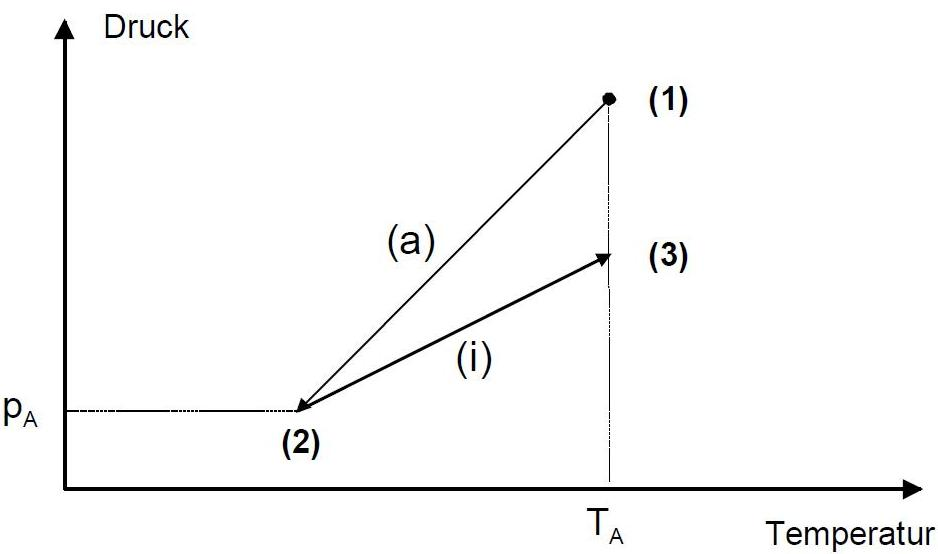
\includegraphics[scale=0.3]{ISE.jpg}
\begin{center}
\caption{adibate Zustandsänderung (Quelle: GP I Skript, Freie Universität Berlin)}
\end{center}
\end{figure}

Bei der Durchführung des Versuchs wird Anfangs ein leichter Überdruck in dem Gefäß erzeugt. Anschließend wartet man, bis der Temperaturausgleich vollzogen ist \(\ T_{1}=T_{A}\). Anschließend öffnen wir ein Ventil, was zum einen zur Folge hat, dass ich das Gas adiabatisch entspannt bis es sich an den Außendruck angepasst hat \(\ (p_{2} = p_{A}) \), und zum anderen verringert sich seine innere Energie und Temperatur. Die Temperaturabnahme kann man mithilfe der {\sc Poisson-Gleichung} berechnen. Als Nächstes erwärmt sich das Gas wieder isochor auf \(\ T_{3} \)auf bis es den Punkt \(\ p_{3} \) erreicht. Dieser Druckanstieg lässt sich durch die allgemeine Zustandsgleichung berechnen. Da die Druck- und Temperaturänderungen relativ klein sind, betrachten wir die Näherung \(\ dp\approx \Delta p\) differentiell. Daras folgt für die {\sc Poisson-Gleichung}:

\begin{equation}
p^{1-\kappa }\cdot T^\kappa =const
\end{equation}

Das totale Differential und eine Umformung liefert uns:

\begin{equation}
\label{10}
(1-\kappa )\frac{dp_{a}}{p}+\kappa \frac{dT_{a}}{T}=0
\end{equation}

Für die isochore Zustandsänderung gilt:
\begin{equation}
\label{11}
\frac{p}{T}=const \notag
\end{equation}
\begin{equation}
\frac{dp_{i}}{T}-p \frac{dT_{i}}{T^2}=0 \hspace{1cm} bzw. \hspace{1cm} \frac{dT_{i}}{T}=\frac{dp_{i}}{p}
\end{equation}

Wenn wir jetzt Gl.\(\eqref{10}\) mit \(\ dT_{i}=-dT_{a}\) in Gl.\(\eqref{11}\) einsetzten, ergibt sich:

\begin{equation}
(1-\kappa ) \frac{dp_{a}}{p}-\kappa \frac{dp-{i}}{p}=0 \notag
\end{equation}

\begin{equation}
\label{12}
\kappa =\frac{dp_{a}}{dp_{a}+dp_{i}}\approx \frac{\Delta h_{1}}{\Delta h_{1}-\Delta h_{3}}
\end{equation}

Dabei ist\(\ h_{1}\) und\(\ h_{3}\) die Höhendifferenz am Manometer am Anfangszustand 1 und Endzustand 3. Gl.\(\eqref{12}\) ist die Messvorschrift der Messmethode von Clement-Desormes. Ein Nachteil ist allerdings, dass aufgrund der niedrigen Druckdifferenz bzw. des kleinen Höhenunterschieds die Messgenauigkeit nicht sehr hoch ist.

\subsection{Die Methode nach Flammersfeld-Rüchert}
Im Gegensatz zu Clement-Desormes Methodehat  Rüchers Schwingungsmethode den Vorteil der höheren Messgenauigkeit. Es wird ein Gasvolumen durch einen beweglichen Kolben abgeschlossen welcher in einem Präzisionsglasrohr schwingt. Das Volumen und der Druck bestimmen dabei die Rückstellkraft und damit die Eigenfrequenz des Kolbens. Diese können wir mithilfe der Adiabatengleichung berechnen. Der Nachteil dieser Methode war die geringe Anzahl der Perioden, wodurch die Messung ebenfalls an Genauigkeit verliert. Flammersfeld verbesserte den Aufbau, indem er durch eine parametrische Selbststeuerung eine stationäre Schwingung erreichte. Er gleichte den Gas- und Energieverlust durch eine kleine Öffnung an der Mittellage des Kolbens aus, durch welchen eine kleine Gasströmung entstand.
Befand sich nun der Kolben unterhalb der Öffnung, verzerrte sich die Schwingung durch die Erhöhung des Gasdrucks. War der Kolben oberhalb des Lochs, ließ sich seine Bewegung durch einen freien Fall mit starker Reibung beschreiben. Entgegen der Erwartungen, war die Störung durch die Reibung sehr viel kleiner und die Eigenfrequenz wurde nur schwach beeinflusst.\\
Nun bilden wir von Gl.\(\eqref{16}\) das totale Differential und erhalten:

\begin{equation}
\frac{dp}{p}+\kappa \frac{dV}{V}=0
\end{equation}

wobei p der Druck ist und V das Volumen. Für die Rückstellkonstante D gilt:

\begin{equation}
D=-\frac{dF}{dx}=-\frac{Sdp}{dx}=\kappa \frac{pS^2}{V}
\end{equation}

Hier entspricht dx und dF der Auslenkung und der Kraft auf den Kolben bzgl. der Ruhelage und S ist die Querschnittsfläche. Als Eigenfrequenz erhalten wir nun:

\begin{equation}
\omega_{0}^2=\frac{D}{m}=\kappa \frac{pS^2}{mV} \hspace{1cm} und \hspace{1cm} \kappa =\frac{4\pi ^2}{\tau ^2} \frac{mV}{pS^2}
\end{equation}

Hierbei sind nun m die Masse und \(\ \tau\) die beobachtete Periodendauer.

\section{Aufgaben}
\subsection{Aufgabe 1}
Bestimmung des Verhältnisses der spezifischen Wärmen \(\ \frac{c_{p}}{c_{v}}=\kappa \) für Luft nach der Methode von {\sc Clement-Desormes}.
\subsection{Aufgabe 2}
Bestimmung des Wertes für \(\ \kappa \)  für ein einatomiges (Argon), ein zweiatomiges \(\ (N_{2}\)) und ein dreiatomiges Gas \(\ (CO_{2})\) durch Messung der Eigenfrequenzen des Gasoszillators.\\
Vergleich der Ergebnisse untereinander und mit den erwarteten Werten aus der kinetischen Gastheorie für ein ideales Gas.

\newpage

\section{Beobachtung und Auswertung}
\subsection{Aufgabe 1}
\subsection{Aufgabe 2}

\section{Fazit}

\end{document}